
\subsection{System Model}
\begin{figure}
\fbox{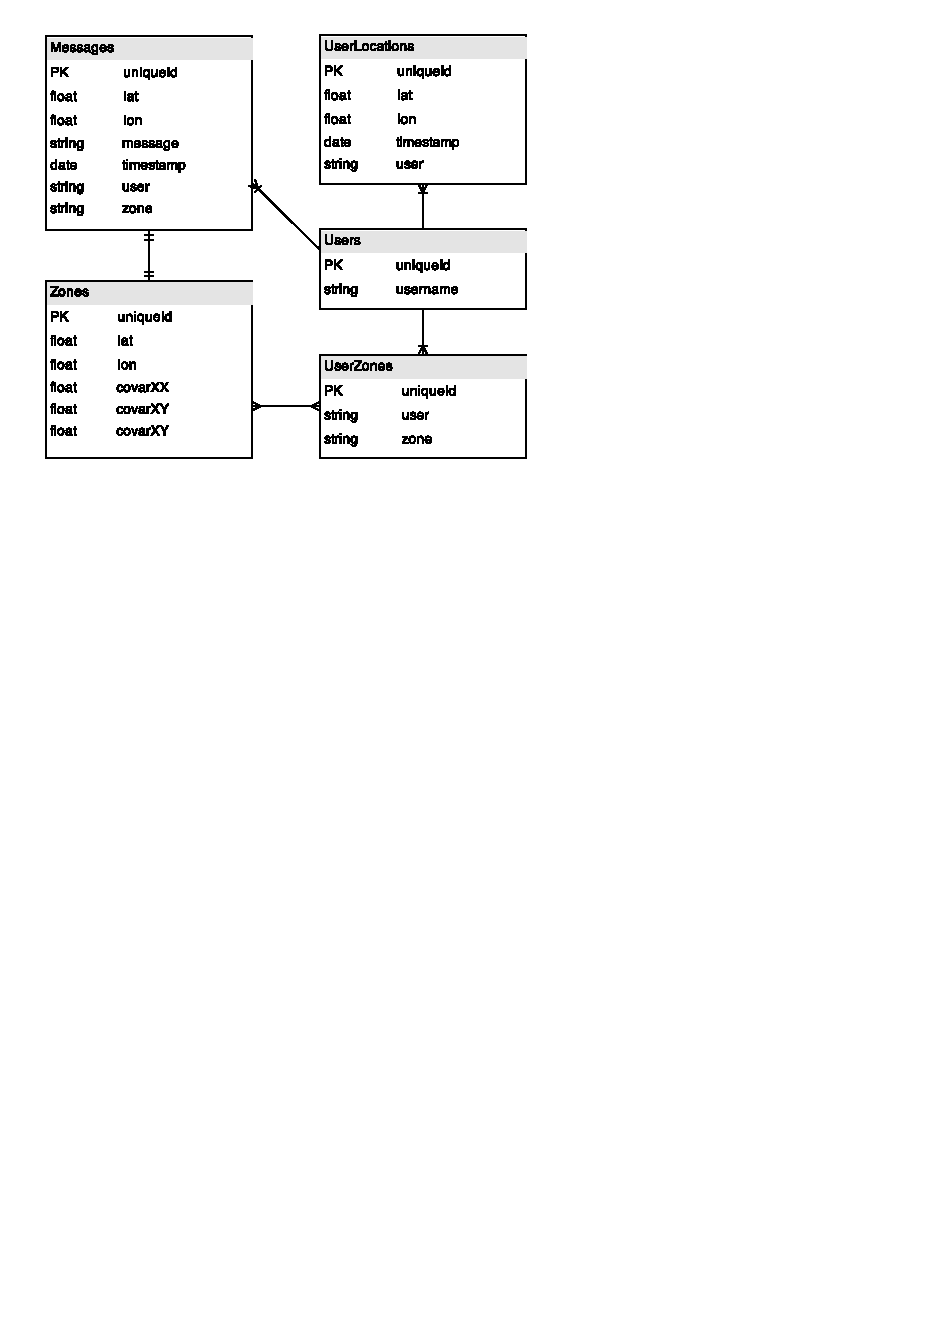
\includegraphics[width=.48\textwidth]{figs/systemModel}}
\caption{GeoChat Database structure.  The user pings the server regularly with their location which is used to determine which zones they should be a part of, and which messages they can see.  Zones behave much like geo-spatial conversation threads, where all messages are public within them.  Zone covariance defines the size and shape of the zones.}
\label{systemModel}
\end{figure}

Our system was implemented with a relatively simple database model shown in figure~\ref{systemModel}.  Firebase allows developers to watch one key on a table for instantaneous updates, and for this reason it is critical to ensure that we can indicate whether a message will be relevant to a user with a single key.  To this end we reorganized our code so that instead of watching a pair of lat/long co-ordinates we instead watch a particular zone.  The zones are calculated by expectation maximization of a gaussian mixture model, discussed in the implementation section.  To facilitate the creation of zones automatically we extract data from firebase onto Parse, where our processing occurs;  discovering zones and getting names for them from Google Places.  Once the algorithm has decided which zones should be created or destroyed the results are written back to the production server where they can change the data users see, as shown in figure~\ref{backendWorkflow}.


\begin{figure}
\fbox{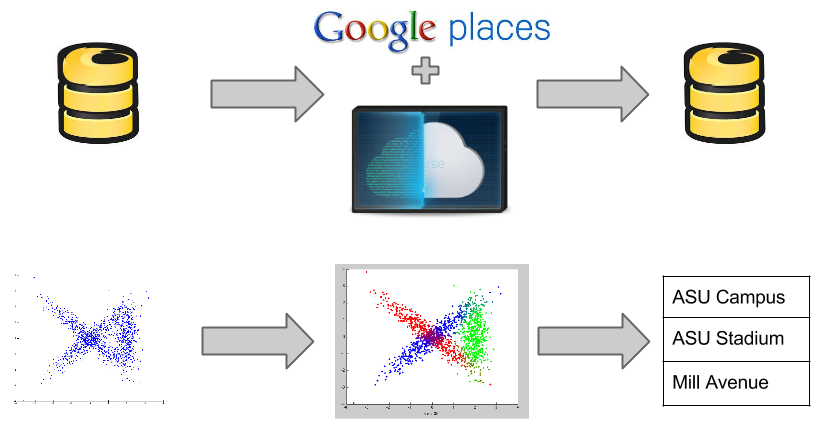
\includegraphics[width=.48\textwidth]{figs/backendWorkflow}}
\caption{Back end workflow.  User locations are added into firebase as a set of latitude and longitude points with no specific significance.  At set intervals data is pulled from firebase into Parse Cloud Code for processing.  Parse then performs expectation maximization and cross-references the located zones with Google Places to name the zone.  Finally these results are written back to firebase so that results can be appropriately tagged.}
\label{backendWorkflow}
\end{figure}

